\documentclass{vgtc}                          % final (conference style)
%\documentclass[review]{vgtc}                 % review
%\documentclass[widereview]{vgtc}             % wide-spaced review
%\documentclass[preprint]{vgtc}               % preprint
%\documentclass[electronic]{vgtc}             % electronic version

\usepackage{mathptmx}
\usepackage{graphicx}
\usepackage{times}
\usepackage{paralist}

%% Add commands for adding author comments:
\newcommand{\wrs}[1]{\textbf{\textcolor[rgb]{0,0,1}{WRS: #1}}}
\newcommand{\pwo}[1]{\textbf{\textcolor[rgb]{0,1,0}{PWO: #1}}}
%%\newcommand{\bill}[1]{}


%% This turns references into clickable hyperlinks.
\usepackage[bookmarks,backref=true,linkcolor=black]{hyperref} %,colorlinks
\hypersetup{
  pdfauthor = {},
  pdftitle = {},
  pdfsubject = {},
  pdfkeywords = {},
  colorlinks=true,
  linkcolor= black,
  citecolor= black,
  pageanchor=true,
  urlcolor = black,
  plainpages = false,
  linktocpage
}

%% If you are submitting a paper to a conference for review with a double
%% blind reviewing process, please replace the value ``0'' below with your
%% OnlineID. Otherwise, you may safely leave it at ``0''.
\onlineid{308}

%% declare the category of your paper, only shown in review mode
\vgtccategory{Research}

%% allow for this line if you want the electronic option to work properly
\vgtcinsertpkg

%% In preprint mode you may define your own headline.
%\preprinttext{To appear in an IEEE VGTC sponsored conference.}

\title{Enhancements to VTK enabling\\ Scientific Visualization in Immersive Environments}

\author{Patrick O'Leary\thanks{e-mail: patrick.oleary@kitware.com}\\ %
        \scriptsize Kitware, Inc., USA%
\and Sankhesh Jhaveri\thanks{e-mail: sankhesh.jhaveri@kitware.com}\\ %
        \scriptsize Kitware, Inc., USA %
\and Aashish Chaudhary\thanks{e-mail: aashish.chaudhary@kitware.com}\\ %
        \scriptsize Kitware, Inc., USA %
\and William Sherman\thanks{e-mail: shermanw@indiana.edu}\\ %
        \scriptsize Indiana University, USA %
\and Ken Martin\thanks{e-mail: ken.martin@kitware.com}\\ %
        \scriptsize Kitware, Inc., USA %
\and David Lonie\thanks{e-mail: david.lonie@kitware.com}\\ %
        \scriptsize Kitware, Inc., USA  %
\and Eric Whiting\thanks{e-mail: eric.whiting@inl.gov}\\ %
        \scriptsize Idaho National Laboratory, USA %
\and James Money\thanks{e-mail: james.money@inl.gov}\\ %
        \scriptsize Idaho National Laboratory, USA %
\and Sandy McKenzie\thanks{e-mail: sandy.mckenzie@kitware.com}\\ %
        \scriptsize Kitware, Inc., USA %
        }


\abstract{Modern scientific, engineering and medical computational simulations and experimental and observational data sensing/measuring devices produce enormous amounts of data.
While statistical analysis is one tool that provides insight into this data, it is scientific visualization that is tactically important for scientific discovery, product design and data analysis.
But these benefits are impeded when the scientific visualization algorithms are implementing from scratch | a time consuming and redundant process in immersive application development.
This process then can greatly benefit by leveraging the state-of-the-art
open source Visualization Toolkit (VTK) and it's community.
But, over the past two (almost three) decades, integrating VTK with a virtual reality environment has only been attempted to varying degrees of success.
In this paper, we demonstrate two new approaches to simplify this amalgamation
of immersive interface with visualization rendering from VTK.
In addition, we cover several enhancements to VTK that provide near real-time updates and efficient interaction.
Finally, we demonstrate the combination of VTK with both Vrui and OpenVR immersive environments in example applications.
} % end of abstract

\keywords{Scientific visualization, immersive environments, virtual reality}

%% ACM Computing Classification System (CCS). 
%% See <http://www.acm.org/class/1998/> for details.
%% The ``\CCScat'' command takes four arguments.

\CCScatlist{ % not used in journal version
 \CCScat{I.3.6}{Computer Graphics}{Methodology and Techniques}{Interaction Techniques};
 \CCScat{I.3.7}{Computer Graphics}{Three-Dimensional Graphics and Realism}{Virtual Reality};
 \CCScat{H.5.2}{Information Interfaces and Representation}{User Interfaces}{Interaction Styles}{Input Devices and Strategies}
}


%% Uncomment below to include a teaser figure.
\teaser{
  \centering
  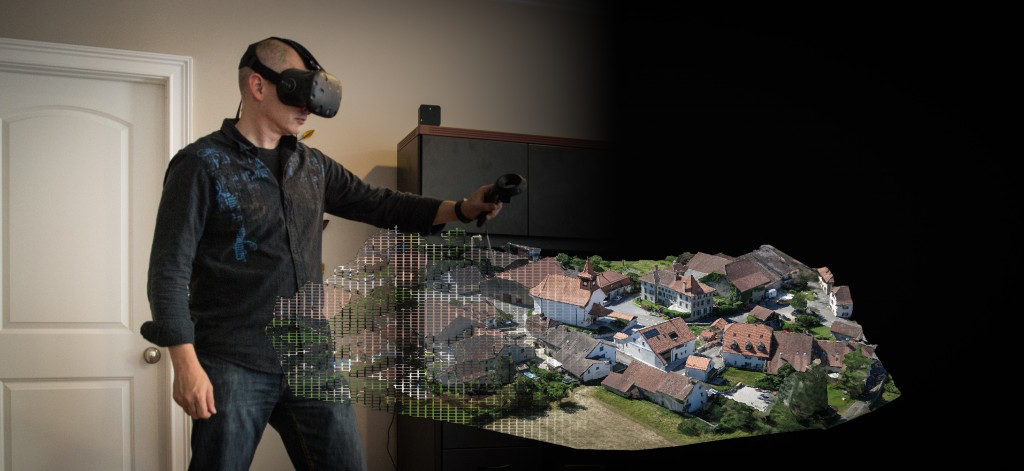
\includegraphics[width=17cm]{images/ViveTownData.png}
  \caption{HTC Vive town data.}
}

%% Uncomment below to disable the manuscript note
%\renewcommand{\manuscriptnotetxt}{}

%% Copyright space is enabled by default as required by guidelines.
%% It is disabled by the 'review' option or via the following command:
% \nocopyrightspace

\begin{document}

\firstsection{Introduction}

\maketitle

There is a growing body of evidence that demonstrates measurable benefits
attained when exploring scientific data using immersive interfaces, such as
molecular research at UNC~\cite{Brooks:1990},
genetics at NCSA~\cite{Brady:1995},
oil well placement at the University of Colorado~\cite{Gruchalla:2004},  confocal microscopy data at Brown University~\cite{Prabhat:2008}, and interdisciplinary immersive visual analytics at the Electronic Visualization Laboratory~\cite{Marai:2016} to name but a few.
While it is not scientifically verifiable, any time scientists
express situations where they "discovered" some relationship in their data
while immersed in a virtual reality (VR) system, we can make the case that the
interface provided a utility that helped them advance their work.

Yet, knowing that there are benefits is only half the equation.
The other half is the cost.
A considerable contribution to the cost | one that is often not
formulated | is personnel time to get data into the VR system.
That time expense is often exacerbated due to a lack of tools that
allow data to be directly imbibed into a virtual environment.

A path that many research teams have taken is to use the established and
feature-rich Visualization Toolkit (VTK).
VTK is a programming-level application programming interface (API) that provides quick access to an expanse
of scientific visualization rendering algorithms, as well as to components
for displaying and interacting with the results on a desktop.
While the concept of combining VTK with VR is sound, the
compatibility of VTK with other rendering software presented a difficult
challenge.  
There were several reasonably successful attempts at this amalgamation,
but in the end, there were either too many inefficiencies to allow the
software to be adequately interactive, or the melding was too fragile to
maintain as VTK and the VR libraries each evolved.

Consequently, the better solution was to adapt VTK to enable it to be
more easily integrated into other rendering systems.
Thus, we adapted VTK by adding new options for rendering.
Rather than always rendering into windows with graphics contexts
created by VTK itself, it is now the possible to "externally" render
into contexts provided by a collaborating system, or even to integrate a
VR system directly into VTK.

Immersive visualization efforts are often associated with research
facilities that provide large-scale VR systems such as CAVEs\texttrademark and
other large-screen walk-in displays.
There is also a growing audience of potential VR users who can now
gain access to immersive interfaces through the new abundance and low-cost
of head-mounted displays (HMDs).
Ideally, there would be one solution to reach both audiences. While this is
technically possible, the consumer systems offer a simpler
approach that will entice many developers to follow that path.
Thus, we offer two approaches, one that addresses the simplier solution
of integrating VTK directly with Oculus or OpenVR and another that allows the integration of VTK with
any full-fledged VR integration library that is capable of interfacing
with CAVE-style and HMD displays.

\textbf{OpenGL context sharing}.
Our \texttt{vtkRenderingExternal} VTK module provides a complete integration API,
including proper lighting, interaction, picking and access to the entire
VTK pipeline.
This, enables simple utilization for application developers using
any OpenGL-based VR Toolkit.

\textbf{VR Toolkit embedding}.
The Oculus and OpenVR VTK modules support several immersive environments directly
without the issues faced by previous work, and it is a complete template
for embedding other VR toolkits within VTK in future work.

\textbf{Enhanced performance}.
As the nature of immersive interfaces, especially HMDs, requires
high-performance rendering, our effort also includes VTK rendering enhancements
including the following:

\begin{compactitem}
\item a new default OpenGL 3.2+ pipeline;
\item dual depth peeling for transparency; and 
\item symmetric multiprocessing (SMP) tools and algorithms.
\end{compactitem}

In the sections that follow, we illustrate how our amalgamation of VTK and VR toolkits support our goals for enhancing scientific visualization through immersive environments.


\section{Related Work}

The use of scientific visualization in immersive environments is simply natural, while tactically important for scientific discovery, product design and data analysis.
There are several high quality scientific visualization virtual reality applications created from scratch using OpenGL directly~\cite{Billen:2008, LaViola:2007, Schulze:2001, Rantzau:1998} including the stunning GPU accelerated hybrid volume and glyph approach for molecular dynamics and other visualizations in the CAVE2~\cite{Reda:2013, Reda:2013a}.
These are certainly exemplary and valuable applications.
However, when building immersive applications, much like desktop applications, with scientific visualization requirements, it is often more efficient to leverage the open-source visualization toolkit (VTK)~\cite{Schroeder:2004}.

Throughout the past two decades, several research teams and developers have integrated VTK with immersive environments to varying degrees of success.
Four fundamental approaches are available to enable VTK in an immersive system:

\begin{compactitem}
\item Geometry transport;
\item OpenGL context sharing;
\item VR toolkit embedding; and
\item OpenGL intercept.
\end{compactitem}

Our recent enhancements to the VTK platform contain solutions for the desired integration that present a number of contributions, and, therefore, we review related work for these areas.

\textbf{\textit{Geometry transport}}
An early approach to VTK--VR integration was the \texttt{vtkActorToPF} library~\cite{Leigh98limbo/vtk}.
In this method, the generation of visualization geometry is decoupled from
the rendering of the geometry (see Figure~\ref{fig:vtkActorToPF}). 
VTK generates the geometry in the form of actors that consist of polygons and properties.
\texttt{vtkActorToPF} transforms these actors into pf-Geodes (nodes) that are included in a Performer (or OpenSceneGraph) scene graph. The geometry is created by VTK, and the scene graph is rendered without VTK. Only geometry is transformed. Cameras, lights, rendering and interaction are not incorporated. Several applications utilized the equivalent \texttt{vtkActorToOSG} for an OpenSceneGraph-based scene graph~\cite{VE-Suite:2016} or directly into OpenGL~\cite{Ohno:2006}. Others have used VTK in a preprocessing step to produce geometries or textures eliminating the need for a direct connection to VTK~\cite{Bivins:2005}.

\begin{figure}[h!]
  \centering
  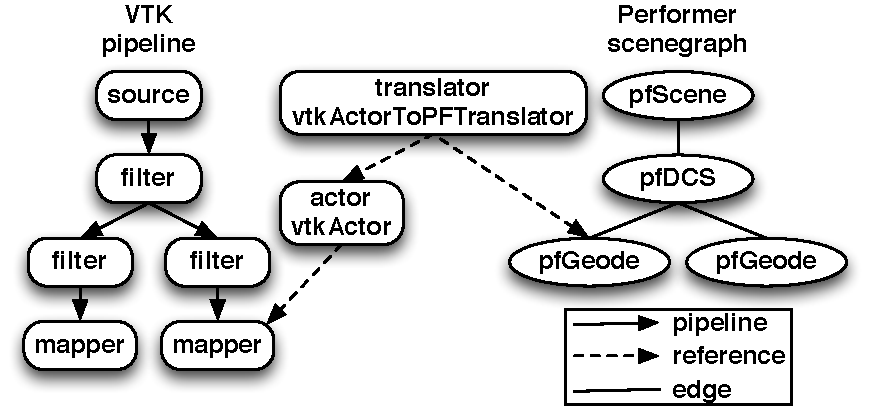
\includegraphics[width=\linewidth]{images/vtkActorToPF.pdf}
  \caption{VTK, vtkActorToPF and Performer interaction diagram. (Recreated from Paul Rajlich~\cite{Leigh98limbo/vtk}.)}
  \label{fig:vtkActorToPF}
\end{figure}

VTK can be used to create, transport and save geometry without rendering. As effective as this approach can be, the loose coupling of VTK and the VR toolkit creates more obstacles than benefits from an application developers perspective, and is, therefore, not built upon by this work.

\textbf{\textit{OpenGL context sharing}} Rather than share just the VTK geometry, the application developer would like to use all of the VTK API from within their immersive application.
In VTK, the renderer and render window classes are responsible for rendering scenes.
VTK creates its own window and associates an OpenGL context with that window to be used by the renderer.
An OpenGL context represents: all of the state, the default framebuffer and everything affiliated with OpenGL with respect to the renderer, window and application.
The application developer seeks to simply share the OpenGL context from the VR toolkit with a third-party rendering software (e.g. Delta3D~\cite{McDowell:2006}, OpenSceneGraph~\cite{Wang:2010} and VTK). 

In previous work, by Sherman et al.~\cite{Sherman:2010} and others, Delta3D
and OpenSceneGraph were quickly modified to instead use windows and associated
OpenGL contexts of a VR integration library such as Vrui~\cite{Kreylos:2006}.  
% in final paper can mention FreeVR.
OmegaLib~\cite{Febretti:2014} software for hybrid reality display environments also implements its own OpenGL context sharing module for VTK, omegaVtk. The AlloSystem~\cite{Amatriain:2009} for the AlloSphere originally had an OpenGL context sharing VTK plugin, but has recently (October 2016) changed to our \texttt{vtkRenderingExternal} VTK module presented in this paper.
These solutions are generally limited in their integration.
Specifically, a rendering library that is unaware of the actual
viewing matrix does not calculate lighting correctly, and
picking input operations do not conform to the shifted rendering. As the VTK API adapts and adds enhancements in time, these implementations are generally locked into to older versions of VTK.

Our \texttt{vtkRenderingExternal} VTK module formalizes this integration, providing lights, interaction and picking connectivity that are lacking in other implementations. The module also offers the application developer complete access to the VTK pipeline.

\textbf{\textit{VR Toolkit embedding}} A similarly time-proven approach is based on the modification of the VTK renderer and render window~\cite{van2000vista, Hannema:2001, Shamonin02vtkcave, Belleman:2003}. 
To render in an immersive environment, derived classes of the
\texttt{vtkRenderer} and \texttt{vtkRenderWindow} are created, which depend on fundamental calls to the VR toolkit.
Thus, VTK-based applications can simply exchange these two items to run on the desktop or the immersive environment.
vtkCave~\cite{Tufo:1999}, for the CAVELib~\cite{CAVELib:2016}, followed by
vjVTK~\cite{Blom:2006} and VR JuggLua~\cite{Pavlik:2012}, for
VRJuggler~\cite{Bierbaum:2001}, created third-party software, essentially
deriving the \texttt{vtkRenderWindow} and \texttt{vtkRenderer} classes. Outside of VTK, lighting and interaction were not shared, which resulted in troublesome behavior.

In this work, we have created two new VTK modules based on either the Oculus~\cite{Oculus:2016} or the OpenVR~\cite{OpenVR:2016} software development kits.
OpenVR is an application programming interface (API) developed by Valve to support its SteamVR ecosystem, compatible with the HTC Vive and other VR hardware~\cite{Road2VR:2015}. Oculus provides software development kits more closely tied to their equipment for mobile, desktop and web VR. The Oculus and OpenVR VTK modules support several immersive environments directly
without the issues faced by previous work, and is a complete template
for embedding other VR toolkits within VTK in future work.

\textit{\textbf{OpenGL intercept}}
A fourth possible means for melding VTK into a virtual environment system
is the \textit{OpenGL intercept} method
~\cite{Humphreys:2001,Humphreys:2002,Zielinski:2014,TechViz:2016,Conduit:2016}, in which middleware is inserted between the application and the graphics card at runtime.
With this technique, closed-source applications can be rendered so that
the head-tracked perspective rendering overrides the internal view matrix
to provide the VR experience.
Thus, this technique enables basic desktop tools to be used with an
immersive interface | albeit a limited interface, given the open-loop nature of
grabbing the rendering, but not connecting back to the parameter interface.
Yet, the perspective rendering alone can be extremely valuable and can allow
scientists, engineers or medical researchers to interact with their desktop
tools in a whole new way. However, many of these methods lack full functionality in the immersive environments, which limits their usefulness to end-users.
Pure OpenGL, without any modifications or additions,  is sure to work using interception.
The difficulty of using intercept methods is that they require more coding
and tagging, and they are not guaranteed to work at all. This is becoming
more difficult with OpenGL 3.0+, especially when using a core OpenGL profile.

In contrast to the OpenGL intercept method, the work in this paper is for the application developer, and there is no intention to eliminate the need to write code. This work aims to make  it easier to develop scientific visualization immersive applications by leveraging VTK.

\textit{\textbf{Enhanced performance}} Near real-time update of scientific visualization metaphors is crucial in immersive environments.
The field has seen several proposed solutions from decoupling rendering, and processing to parallel visualization~\cite{Bryson:1996, van2000vista}.
This effort stands apart from all these previous efforts. Valiant
as they were, the efforts were ultimately lost to time, as VTK has continued to
evolve, making it difficult for tacked-together components to remain in
sync with the API.
Rather, by providing rendering access from within the VTK API itself, new
tools can rely on a stability that has not been available for techniques
that perform functions outside the bounds of the API design. Often, such techniques access
internal features that do not have the assurance of stability.
As a commercially supported open-source tool, VTK's rendering performance is
continually being advanced.
VTK has been around since 1993 with over one hundred thousand repository commits from over two-hundred and fifty contributors.
Having the latest algorithm implementation requires the use of the existing implementation in VTK or calls for the algorithm's contribution to VTK.

We present recent enhancements to VTK that significantly impact immersive
environment application development. The OpenGL 3.2+ pipeline, described in Hanwell et al~\cite{Hanwell:2015}, provides the most dramatic improvement in performance. We have supplemented this work with Bavoil and Myers dual depth peeling~\cite{Bavoil:2008}, as well as symmetric multiprocessing (SMP) tools and algorithms, to address the performance issues for transparent geometry and computationally intense algorithms (e.g., isosurfaces).

Finally, our work will eventually allow application developers to leverage portable threaded data parallel algorithms capable of running on next generation hardware from VTK-m~\cite{Moreland:2016}. VTK-m has shown impressive results in its first two years of development. As the number of filters available in VTK-m's repository grows, the plan is to make them available in the next major release of VTK. Thus, if VTK-m is contained in VTK, then applications developed using the integrations described in this paper can use it.

\section{Approaches}

To achieve broader usage it is important to require few if any changes to either the VR toolkit or the third party scientific visualization software, and to work as close as possible to the standard application development workflow.
For VTK, this was accomplished by adding new features that fit within the existing architecture. 
VTK provides a well-defined rendering pipeline through the \texttt{RenderWindow}, \texttt{Renderer}, \texttt{Camera}, \texttt{Actor}, and \texttt{Mapper} classes.
This precise pipeline definition and clear-cut API of VTK enabled us to primarily build upon
existing code.
In the next section we cover details on these components from the architecture point of view.
In the implementation sub-section, we provide in-depth details of features we implemented to support configurable immersive scientific visualization applications. 

\subsection{OpenGL context sharing}

Traditionally, VTK creates and manages its own OpenGL context and the data objects within the scene.
The objective of this work is to bring the high-quality scientific visualization computing and rendering capabilities of VTK to virtual reality environments in a way that is easier to develop and maintain.
By bringing VTK into virtual environments created by interface-specific tools such as GLUT, VRUI, and FreeVR, we are providing the tools necessary to build interactive, 3D scientific visualizations to the developers of the virtual reality community.

\subsubsection{Architecture}

Integrating VTK into external rendering systems required overriding some of the behavior of the \texttt{vtkRenderWindow}, \texttt{vtkRenderer}, and \texttt{vtkCamera} classes.
A \texttt{Renderer} is attached to a \texttt{RenderWindow}, a \texttt{Mapper} to an \texttt{Actor}, and a \texttt{Camera} to a \texttt{Renderer}.
In a typical VTK application the \texttt{RenderWindow} class is responsible for creating a rendering context, and defining width and height of the visualization viewport.
The \texttt{Renderer} class is responsible for rendering one-or-more
\texttt{Actor}s and managing the viewport within the \texttt{RenderWindow}.
The \texttt{Actor} class is a drawable entity, which uses a \texttt{Mapper} to render specific data within a \texttt{Renderer}.
Figure \ref{fig:vtkRenderPipeline} shows the classes and interactions between them.

Each of these components has its corresponding derived classes that implement the API using OpenGL, VTK's underlying graphics API.
Using OpenGL provides VTK with the ability to use hardware acceleration that ultimately leads to better visualizations and near real-time performance as required by many interactive applications especially ones that are designed for immersive environments.
Each component of VTK participates in a specific way and communicates with other components via the public API.
For instance, the \texttt{RenderWindow} typically creates the context in which
\texttt{Renderer} draws drawable entities, i.e. \texttt{Actor}s.
%A \texttt{RenderWindow} can have one or more \texttt{Renderer}s.
%Each \texttt{Renderer} can make a decision on whether or not it should reset the buffers such as color or depth to its initial state while rendering one-or-more actors. 

\begin{figure}[h!]
  \centering
  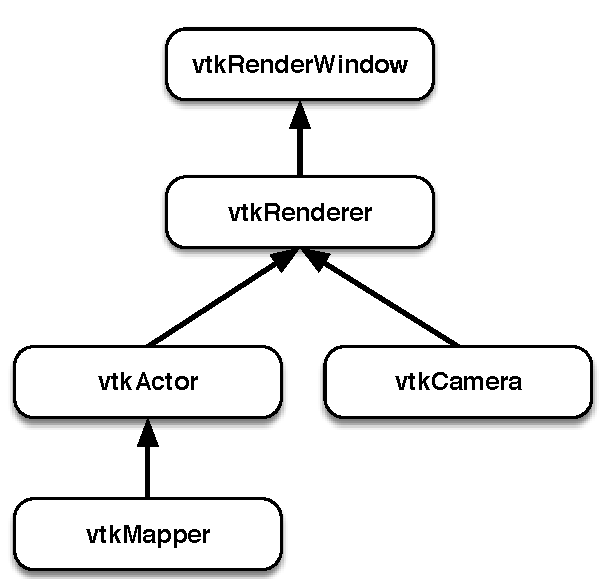
\includegraphics[scale=0.5]{images/vtkRenderPipeline.pdf}
  \caption{vtkRenderWindow, vtkRenderer, vtkCamera, vtkActor, and vtkMapper interaction diagram.}
  \label{fig:vtkRenderPipeline}
\end{figure}

Since \texttt{vtkRenderWindow} typically creates the context, and \texttt{vtkRenderer} controls the rendering of individual objects in a scene of a given viewport, the rendering pipeline is constructed with properties and other attributes set specifically to support this most general use case.
However, in the case of external environments, the context is created outside of VTK, and non-VTK graphical elements (such as the GUI) may be rendered before or after the VTK rendering.
In addition, the environment may render its own visualization objects in the same context.
To handle this situation, we have introduced a new module in VTK called \texttt{vtkRenderingExternal} that comprises four new classes: \texttt{vtkExternalOpenGLRenderWindow}, \texttt{vtkExternalOpenGLRenderer}, \texttt{vtkExternalOpenGLCamera} and \texttt{ExternalVTKWidget}. 

\textbf{\texttt{vtkExternalOpenGLRenderWindow}} - This class is an extension to
the \texttt{vtkGenericOpenGLRenderWindow} class, which provides a
platform-agnostic VTK OpenGL window.
The external render window class prevents a new VTK render window from being
created and, instead, uses an existing OpenGL context.
It is also responsible for fetching stereo parameters from the parent OpenGL
application and setting them on the VTK pipeline.

\textbf{\texttt{vtkExternalOpenGLRenderer}} - This class derives from
\texttt{vtkRenderer} and provides all of its features and functionalities. The
external renderer offers an API that prevents it from clearing the OpenGL color
and depth buffers at each frame. This ensures that the main application holds
control over the OpenGL context and preserves rendered elements in the scene, of
which VTK is unaware.

\textbf{\texttt{vtkExternalOpenGLCamera}} - This class inherits
\texttt{vtkCamera} and provides the ability to set the projection and modelview
matrices on the camera. This allows the external rendering framework to easily
set the view and orientation on the VTK camera. The external camera also uses
this scene information to compute accurate lighting matrices.

\textbf{\texttt{ExternalVTKWidget}} - This is a collective implementation that
provides a plug-and-play approach to the \texttt{vtkRenderingExternal} module.
It allows the consumer application to use all the new classes as described above
in just one step. The overarching application needs only to instantiate this
class to use VTK's external rendering capabilities. The
\texttt{ExtenalVTKWidget} creates a new external render window or uses one
provided to it from the external library / application.

\subsubsection{Implementation}

One of the most important prerequisites of this work was seamless stereo rendering and user interaction between the rendering native to the base virtual reality toolkit and the rendering embedded in VTK. 

\textbf{\textit{Stereo Rendering}} The OpenGL context maintains the state machine in which OpenGL commands change the state of the system or query a particular state as needed.
To support stereo, we utilized the OpenGL context, set by the VR toolkit, to determine the type of stereo (Quad Buffer, Side-by Side, or Top-Bottom stereo) and simply render using the OpenGL context, which sets active buffer, stenciling, etc.
This is set only once, immediately after the context has been created, and is maintained by the VR toolkit over time. 

\textbf{\textit{2D and 3D Interface Widgets}} In most cases, VTK elements will not be the only objects in a scene.
There will probably be some GUI elements that will also be rendered in addition to the VTK elements.
Thus, the VTK rendering will be mixed with other OpenGL elements.
The new \texttt{ExternalRenderer} class does not clear the depth or color buffers, leaving that to the display integration library or application.
The depth buffer can then act to allow OpenGL elements to be mixed (composited) in three-space with closer elements occluding farther ones.

\textbf{\textit{User Interactions}} Generally, in the case of a VR toolkit, interaction such as navigation in the scene space, grab, and rotation of various scene objects are handled by the VR integration library (e.g., Vrui).
VTK has its own classes and methods for interaction and scene object manipulation.
To synchronize the navigation in these two systems, the \texttt{vtkExternalOpenGLCamera} class has been added.
This class empowers the external application to manage camera interaction for VTK objects.
We added a GL query in the external renderer, which uses the GL state system to get the projection and modelview transformation matrices.
These two matrices determine the location and orientation of the user's eye
(camera) in the scene.
The \texttt{vtkExternalOpenGLRenderer} sets these matrices on the \texttt{vtkExternalOpenGLCamera}.
Setting these matrices directly on the camera leaves the camera parameters such as position, focal point, and view up direction to incorrect values, Therefore, we compute appropriate viewing coordinates for the camera by multiplying the modelview matrix with the camera initial default position in the OpenGL coordinate system. 
Once, everything is set on the camera, the navigation and lighting works as expected by the user.

The application itself handles the secondary kind of interactions such as interactive slicing and clipping of the scientific datasets.
VTK provides classes (filters) to perform thresholding, clipping, slicing, etc.
These filters take parameters such as thresholding value, slicing position, and clip position. 
In our implementation, the application receives the 6-DOF tracker position data, and, based on the mode of the application, uses this information to set appropriate values on a specific filter.
For example, the left hand controller might be used to position the clipping plane.
This integration is straightforward because our module makes the coordinate system consistent between the two rendering systems.

\subsubsection{Enabling \texttt{vtkRenderingExternal}}

This work has been merged into the VTK as of release 7.0 available at
\url{http://www.vtk.org}.
To enable this module when compiling VTK with \texttt{CMake},
set \texttt{Module\_vtkRenderingExternal} to \texttt{ON} (default is \texttt{OFF}).

\subsection{VR Toolkit Embedding (Oculus and OpenVR)}

The potential VR user base has grown profusely with the emerging
proliferation of consumer-level HMD VR displays along with their associated
software ecosystems, such as Valve's SteamVR.
For developers who are willing to specifically target this audience, perhaps
excluding users of CAVE-style VR displays, a simpler VTK-VR alternative is
also available.
The trade-off | for developers who don't already have expertise in a
full-fledged VR integration library | is avoiding the programming of
the alternative VR integration library, and immediately gaining access
to HMDs compatible with OpenVR, but not to other VR display systems.

To enable using consumer VR devices with VTK, we created Oculus and OpenVR modules in VTK .
Our goal is to allow VTK programs to use consumer VR devices with few changes, if any, and to support natural interaction when using them.
If you link your executable to the \texttt{vtkRenderingOpenVR} or \texttt{vtkRenderingOculus} modules, the object factory
mechanism will replace the core rendering classes (e.g.,
\texttt{vtkRenderWindow} and \texttt{vtkRenderer}) with the VR specialized versions in VTK.  This also entails changes to the 
interaction model as VR and VR devices are naturally 3D in nature with single and multi-touch events occurring in 3D space as 
opposed to the more traditional 2D screen space. To this end we created new classes that support natural picking and interaction given 3D 
input devices.

One example of this low barrier of entry is incorporating consumer VR support into the latest release of ParaView. With minimal changes to ParaView we are enabling researchers to load up existing visualizations in ParaView and send them to VR to explore them with the Vive or Rift. Researchers can bounce back and forth between the traditional desktop and consumer VR experiences with the press of a button. This type of integration targets our goal of providing a solution with a low barrier of entry.

\subsubsection{Implementation}

The integrated VR support contains the following classes as drop-in replacements in VTK.

\textbf{\texttt{vtkOpenVR/OculusRenderWindow}} - This is a derived class of the RenderWindow class.
This class holds the initialization and main interfacing to the consumer VR toolkit. 

\textbf{\texttt{vtkOpenVR/OculusRenderer}} - This is a derived class of the Render class.
Consumer VR devices exist in real world coordinates such as meters, while the world coordinate system of a visualization could be anything from microns to AUs. As such, movements in the real world need to be scaled and translated into reasonable movements in the visualization's world coordinates. The \texttt{vtkOpenVR/OculusRenderer} class computes a reasonable scale and translation which are then used in computing the view and input device transforms. 
It also sets an appropriate default clipping range expansion.

\textbf{\texttt{vtkOpenVR/OculusCamera}} - This is a derived class of the Camera class. \texttt{vtkOpenVRCamera} gets the matrices from the VR library to use for rendering and integrates them with the model, view and world matrices from the visualization. It contains a scale and translation that are designed to map world coordinates into the HMD space.
Accordingly, the application developer can keep world coordinates in the units best suited to their problem domain, and the camera will shift and scale into units that make sense for the HMD.

\textbf{\texttt{vtkOpenVR/OculusRenderWindowInteractor}} - VTK is designed to pick and interact based on two-degrees of freedom, desktop X and Y mouse/window coordinates.
In contrast, VR provides X, Y and Z 3D world coordinates and 3D orientations.
The \texttt{vtkOpenVRRenderWindowInteractor} class catches controller events and converts them to mouse/window events.
In addition, this class also stores the world coordinate positions and orientations for the styles or pickers that need them.
\texttt{vtkOpenVRRenderWindowInteractor} supports multiple controllers through the standard PointerIndex apfsproach that VTK uses for multi-touch.

\textbf{\texttt{vtkInteractorStyle3D}} - In concert with the VR specialized \texttt{vtkRenderWindowInteractor} classed, we derived the \texttt{vtkInteractorStyle3D} class
to use 3D world coordinate events to manipulate \texttt{Actor}s, and handle multi-touch 3D events such as scaling or translating the world to real transforms.
This class provides a common grab-and-move style of interaction that is common to OpenVR and other VR toolkits.

\textbf{\texttt{vtkPropPicke3D}} - Finally, the derived \texttt{vtkPropPicke3D} class determines what \texttt{Actor}s or \texttt{Prop}s VTK picks.
Note that \texttt{Prop} is an abstract superclass for any object that can exist in a rendered scene (either 2D or 3D), and defines the API for picking, LOD manipulation, and common instance variables that control visibility, picking, and dragging.
The \texttt{vtkPropPicker3D} class uses the 3D world coordinate from a VR device as the picking value as opposed to using a 2D event and intersecting a ray, which is slower.

These derived classes work from within VTK to provide seamless access to cameras, lighting, interaction and the complete VTK pipeline.

\subsubsection{Enabling the OpenVR and Oculus Modules}

To use VTK with Oculus or OpenVR support, first download VTK 7.1 or later from the VTK
repository on GitHub (see \url{http://www.vtk.org}).
To enable these modules, use \texttt{CMake} to set \texttt{Module\_vtkRenderingOpenVR} or \texttt{Module\_vtkRenderingOculus} to \texttt{ON} (default is \texttt{OFF}).
The \texttt{CMake} build process will prompt you for some external libraries including Simple DirectMedia Layer 2 (SDL2) and the OpenVR or Oculus SDK as appropriate.
Ensure you build an optimized version of VTK to maximize performance while using these new capabilities.

\subsubsection{Future Developments}

The consumer VR support is currently in the beta phase and has been tested on the HTC Vive and Oculus Rift. Moving forward, we look to add support for the features such as overlays, which provide support for user interface components. We also expect to include more event interactions, Oculus touch controller support, and measurement widgets.

\subsection{Performance enhancements}

VTK is one of the most commonly used libraries for visualization and computing in the scientific community.
Primarily written in C++, VTK provides classical and model visualization algorithms to visualize structured, unstructured, and point data sets on desktop, mobile, and web environments.
VTK provides state-of-the-art implementations accessible via an API call.
The benefit in using VTK comes from the fact that having the latest algorithm implementation simply requires using the existing implementation from the
open source, community driven VTK repository or contributing one.

To allow VTK to function at levels needed for head-tracked rendering,
many other enhancements have been added to the overall VTK system:
using modern OpenGL,
rendering transparencies with dual-depth peeling, and
expanding the use of multi-threading.

\subsubsection{OpenGL 3.2+}

The legacy rendering code in VTK is a group of implementation modules collectively called ``OpenGL."
Through a grant from the National Institutes of Health, the OpenGL group has
been rewritten as a drop-in replacement set of implementation modules
collectively called ``OpenGL2".
This work aims to support rendering on modern graphics cards~\cite{Hanwell:2015}.

The results have been nothing short of spectacular.
Polygon rendering demonstrates a ten fold speedup for first frame rendering followed by a two-hundred fold speed up for subsequent frames for one to thirty million triangles.
The previous volume rendering was also graphics processing unit (GPU) aware, and, thus, the improvement is a modest but substantial two fold speedup. 

To realize these performance enhancements, VTK now uses an OpenGL 3.2+ context, which is available on fairly low end modern GPUs.
However, for those application developers using the X11 window system on a Mac OSX system, xQuartz does not currently provide a suitable OpenGL context.
But, as xQuatrz utilizes newer versions of Mesa going forward, we expect future versions will eventually meet the OpenGL2 requirements.

\subsubsection{Dual-Depth Peeling}

As we developed several example programs leveraging the \texttt{vtkRenderingExternal} module, we found that the rendering performance slowed as transparency was introduced into the scene. We have developed a dual-depth peeling algorithm to overcome this issue.

In OpenGL, polygons are broken up into fragments through the rasterization process.
Each fragment corresponds to a pixel.
An OpenGL fragment shader is a customizable program that determines the color of a fragment where all fragments for a single pixel are blended to determine the final color of the pixel.
Composing multiple translucent fragments into a single pixel must be done carefully.
There are three common strategies to this composition:

\begin{compactitem}
\item \textbf{Simple Alpha Blending} - The fragments are processed (blended using just alpha) in random order.
  It is very fast, but provides unpredictable and generally incorrect results.
\item \textbf{Sorted Geometry} - Geometry must be resorted each time the camera moves using \texttt{vtkDepthSortPolyData}.
  Sorting is an expensive (slow) operation, but provides generally consistent results with some artifacts where primitives overlap.
\item \textbf{Depth Peeling} - Extract and blend fragments in a multipass render, and, therefore, requires multiple geometry render passes.
\end{compactitem}

VTK by default uses depth peeling.
To enhance rendering performance with transparency we implemented \texttt{vtkDualDepthPeelingPass}, which was originally proposed by nVidia in 2008~\cite{Bavoil:2008}.
Dual-depth peeling extends traditional depth peeling by extracting two layers of fragments per-pass: from the front and back simultaneously.
Uses a two-component depth buffer to track of peel information and three types of geometry passes:

\begin{compactitem}
\item \textbf{InitializeDepth} - Initializes buffers using opaque geometry information.
\item \textbf{Peeling} - Repeated pass that extracts and blends translucent geometry peels.
  It extracts both near and far peels while blending far peels into accumulation buffer.
\item \textbf{AlphaBlending} - An optional pass to clean up unpeeled fragments and used with occlusion thresholds.
\end{compactitem}

This algorithm provides a two fold speedup for compositing in the appearance of transparent geometry.

\subsubsection{vtkSMPTools}

The field of parallel computing is advancing rapidly due to innovations in GPU and multicore technologies.
The VTK community is working to make parallel computing for scientific visualization easier by introducing \texttt{vtkSMPTools}, an abstraction for threaded processing which uses different libraries such as TBB~\cite{TBB:2016}, OpenMP~\cite{OpenMP:2016} and XKaapi~\cite{Gautier:2013}.
The typical target application is coarse-grained shared-memory computing as provided by mainstream multicore, threaded CPUs such as Intel's i5 and i7 architectures.

For several of the example programs utilizing the \texttt{vtkRenderingExternal} module, we leveraged a new contouring algorithm in VTK that is readily parallelizable using \texttt{vtkSMPTools} and still incredibly efficient in serial mode, called \texttt{vtkFlyingEdges2D} and \texttt{vtkFlyingEdges3D}.
While the OpenGL2 group improves rendering performance, \texttt{vtkSMPTools} can be used to enhance the geometry generation performance for scientific visualization.


\section{Results}

To demonstrate the utility our VTK enhancements provide scientific
visualization efforts and to test various use cases, we have implemented three kinds of
applications for the \texttt{vtkRenderingExternal} approach as well as
a simple example using \texttt{vtkOpenVR}.
Using the Vrui VR integration library, we created the following applications:
GeometryViewer, VolumeViewer and MooseViewer.
As the names suggest, GeometryViewer enables end users to load geometry files from a file; VolumeViewer renders a structured dataset using the GPU based volume rendering technique in VTK; and MooseViewer renders a multi-block unstructured dataset as a geometry or a volume, depending on the end user's interactive selections.

\subsection{Immersive Environments}

A variety of immersive environment display styles exist, from HMDs, to low-cost IQ-stations~\cite{Sherman:2010}, to four- or six-sided CAVE\texttrademark systems. Immersive applications need to support a large number of immersive environments, as each has its strength and applicability in real-world scenarios. We have tested our work in the following virtual environments: 

\begin{compactitem}
\item a four-sided CAVE\texttrademark;
\item a low cost IQ-station; and 
\item an HTC VIVE HMD.
\end{compactitem}

In the first two cases, the \texttt{vtkRenderingExternal} module was used with the Vrui VR toolkit to provide the configuration necessary to run the application. For HTC VIVE, we leveraged \texttt{vtkOpenVR}. 

\subsection{Vrui Implementation}

The task of a VR toolkit is to shield an application developer from the particular configuration of an immersive environment, such that applications can be developed quickly and in a portable and scalable fashion. There are three important parts of this overarching goal: encapsulation of the display environment, encapsulation of the distribution environment and encapsulation of the input device environment.

The Vrui VR toolkit supports fully scalable and portable applications that run on a range of immersive environments, starting from laptops with touchpads, to desktop environments with special input devices such as space balls, to full-blown immersive VR environments ranging from single-screen workbenches to multi-screen tiled display walls or CAVE\texttrademark systems. Applications using the Vrui VR toolkit are written without a particular input environment in mind, and Vrui enabled immersive environments are configured to map the available displays and input devices to the application, such that they appear to be written natively for the environment. For example, a Vrui application running on the desktop should be as usable and intuitive as any 3D application written specifically for the desktop.

We developed some example applications that serve as validation of this effort. There is an example within the VTK source tree for the \texttt{vtkRenderingExternal} module that renders a VTK sphere in an OpenGL Utility Toolkit (GLUT) window. We also developed three advanced applications that illustrate VTK rendering within a Vrui created OpenGL context. These applications exhibit varying capabilities of the VTK infrastructure leveraged by the \texttt{vtkRenderingExternal} module. 

\subsubsection{GeometryViewer}

GeometryViewer~\cite{GeometryViewer} reads and renders a Wavefront (.obj) file that defines a geometry.
It reads the file using the standard \texttt{vtkOBJFileReader} that creates \texttt{vtkPolyData} from the geometry.
The \texttt{vtkPolyData} is then mapped, using the polydata rendering pipeline in VTK, as a \texttt{vtkActor} object.
The main menu of the application allows the user to center the geometry to the screen as well as to change its representation.
The \textit{Center Display} button calculates the transformation from the current camera position and direction to the center position.
The \textit{Rendering Options} sub-menu allows the end user to change the opacity of the \textit{vtkActor} object, leveraging our work on dual depth peeling, as well as its representation to either the points, the wireframe or the surface.
In addition to VTK level modifications, the application has support for OpenGL level widgets (e.g., \texttt{glClipPlane}).
This shows that native OpenGL operations can also be interactively performed when using the VTK rendering pipeline.

\begin{figure}[h!]
 \centering
 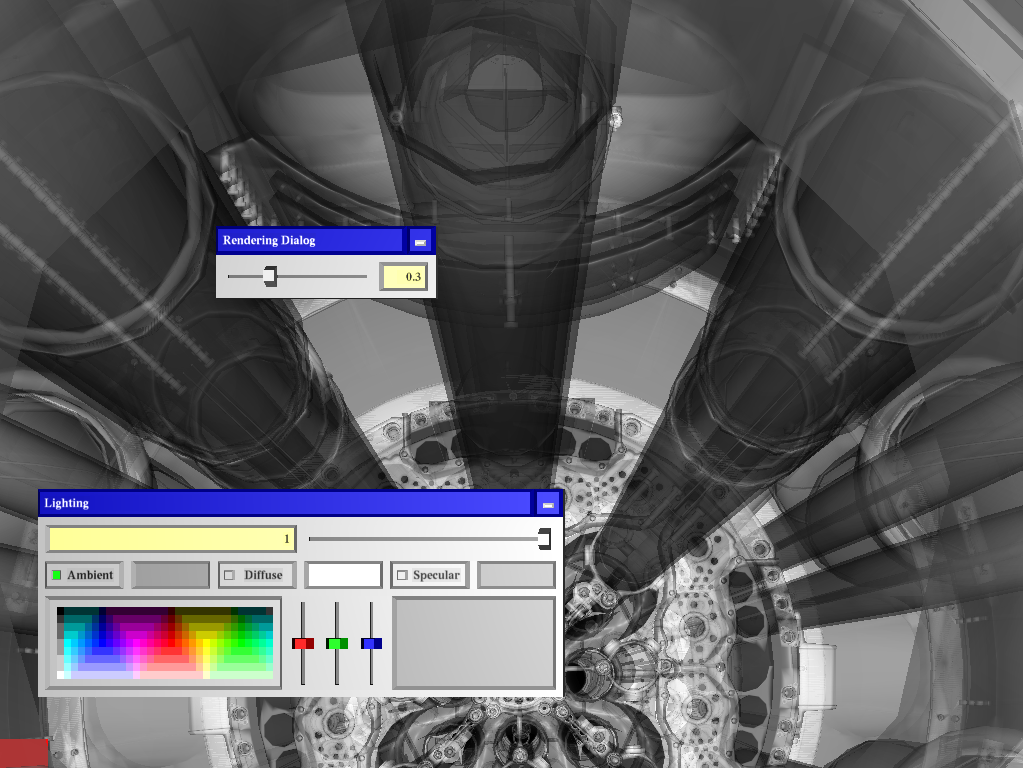
\includegraphics[width=3.in]{images/vessel.png}
 \caption{Geometry representing Idaho National Laboratory's Advanced Test Reactor (ATR) core. The geometry is used to virtually understand maintenance processes in this extreme environment.}
 \label{fig:vessel}
\end{figure}

In Figure~\ref{fig:vessel}, we show the Vrui user interface (UI) with the ``\textit{Rendering Options}" dialog that allowed us to adjust the transparency of the Advanced Test Reactor (ATR) core. In addition, we used the Vrui UI to build an interface for the lighting color that seamlessly maps between Vrui and VTK.

This example has the functionality contained in the integration between Vrui and Delta3D presented in Sherman et al.~\cite{Sherman:2010}. Both applications were simple to develop, but the performance of GeometryViewer is faster, especially when rendering transparent geometry. In addition, GeometryViewer integrates the lighting between the VR toolkit and VTK, in contrast to the Vrui/Delta3D integration, which requires modification to the material textures to provide false lighting.

\subsubsection{VolumeViewer}

\begin{figure}[h!]
 \centering
 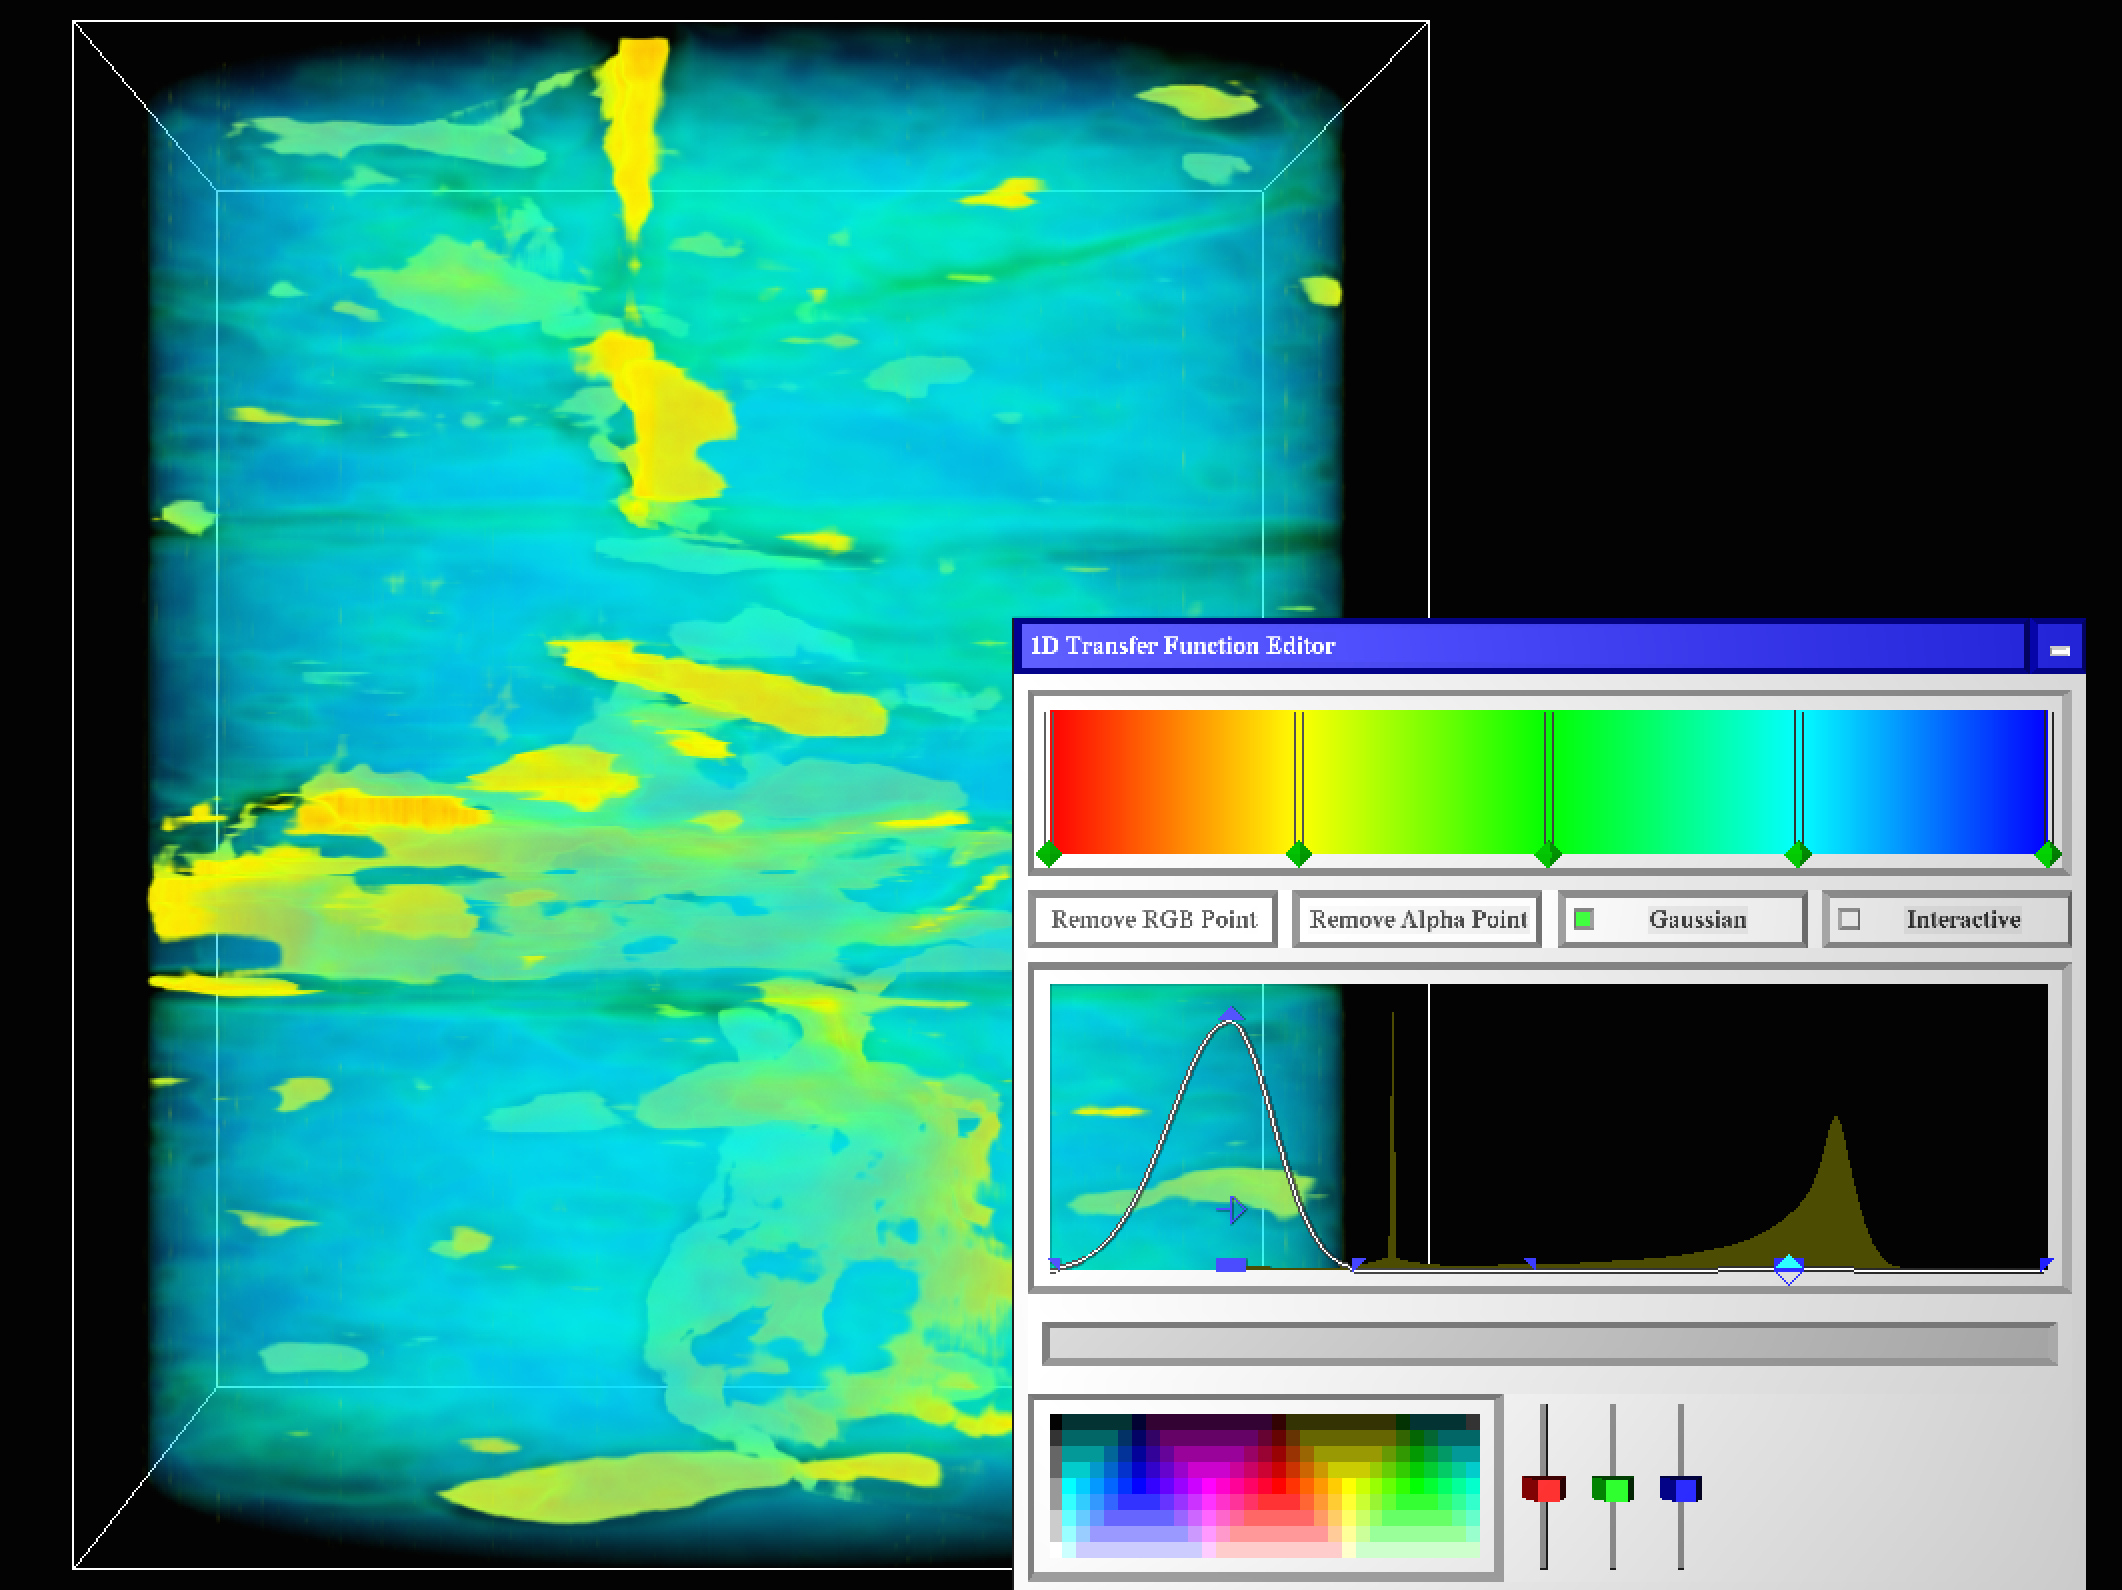
\includegraphics[width=3.in]{images/rock-transferfunction.png}
 \caption{A digitized well ``rock" core. The yellow isosurfaces isolate the oil trapped within the shale rock.}
 \label{fig:volume}
\end{figure}

VolumeViewer~\cite{VolumeViewer} reads and renders VTK ImageData (.vti) files that define structured points datasets.  The application instantiates a pipeline that allows volume rendering of the dataset. Several pre-defined color maps help to change the mapping of scalar values to colors. A ``\textit{Transfer Function}" editor allows changes to be made to the color and opacity of the rendered volume.

Figure~\ref{fig:volume} depicts our implementation of a ``\textit{Transfer Function}" editor using the Vrui UI. In addition, we leveraged \texttt{vtkFlyingEdges3D} to display the oil isosurfaces in yellow and blend the results in the volume.

Widgets such as ``\textit{Isosurfaces}", ``\textit{Contours}" and ``\textit{Slice}" provide VTK level operations that can be carried out on the dataset. To circumvent possible interaction problems when dealing with large datasets, a low-resolution mode is provided that downsamples the dataset. This lets the end user fulfill actions quickly and then revert back to the full size, when they are ready to visualize the complete dataset.

Immersive volume visualization applications are fundamental for a number of scientific research domains, and it is not surprising that there exists a number of partial solutions in the public domain. VolumeViewer has similar features contained in both Visualizer~\cite{Billen:2008} and Toirt Samhlaigh~\cite{O'Leary:2008}. Both applications use complex, from scratch, OpenGL algorithms that were time-consuming to develop. Visualizer uses a standard GPU OpenGL Shading Language (GLSL) shader-based ray-casting algorithm. Toirt uses an octree-based space-skipping GPU GLSL shader-based view-aligned algorithm to provide higher performance on larger volumes. In contrast, VolumeViewer requires less than a hundred lines of VTK API to implement roughly the same GPU GLSL shader-based ray casting used in Visualizer. The performance of VolumeViewer is equal to or exceeds that of the other tools. In addition, by modifying a line or two of VolumeViewer code, the application can accept data from any of the hundred-plus supported scientific data formats|a feat that would require the implementation of readers, data structures and algorithms in either of the other two applications.

\subsubsection{MooseViewer}

MooseViewer~\cite{MooseViewer} reads and displays Moose framework~\cite{Gaston:2015, MooseFramework} ExodusII (.ex2, .e) files in immersive environments. The application uses \texttt{vtkExodusIIReader} to read geometry defined in ExodusII files as well as associated attributes (e.g., temperature, burnup, etc.). The application permits only user-selected variables to be loaded as data arrays, thus reducing memory overhead. A ``\textit{Color By}" sub-menu is dynamically populated with user-selected variables. The sub-menu maps the chosen variable scalars to colors using the selected color map.
An interesting capability of the application is animation of the dataset over time.
The ``\textit{Animation}" dialog helps play through the time steps with controls for looping and stepping through the time steps.

In Figure~\ref{fig:fuelpin}, we see surface geometry colored by the selected temperature attribute animated using the ``\textit{Animation}" dialog.

Like Visualizer~\cite{Billen:2008}, MooseViewer provides a number of scientific visualization techniques for simulation data, but MooseViewer was created in weeks. Enhancements are added by simply plugging in alternative VTK algorithms to increase/scale performance.  Although it is focused on the ExodusII file format, MooseViewer makes accepting data from other scientific data formats a simple task. MooseViewer outperforms Visualizer using the VTK OpenGL 3.2+ rendering pipeline, but pure rendering performance fails to highlight the unique immersive-specific level-of-detail algorithms in Visualizer. Visualizer is a fantastic immersive application. If an end user has data in one of its accepted formats, we encourage that person to leverage some of the unique Visualizer features.

\begin{figure}[h!]
 \centering
 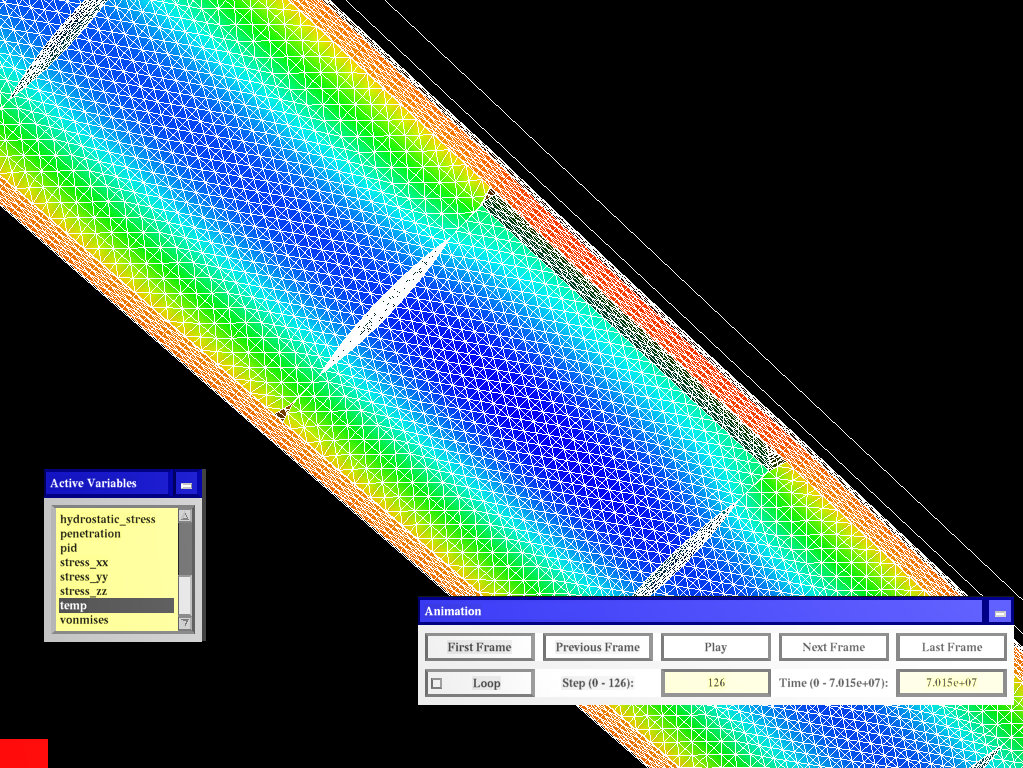
\includegraphics[width=3.in]{images/fuelpin.png}
 \caption{A MOOSE Framework application, BISON, simulates a nuclear pin with missing cladding on one of the fuel pellets.}
 \label{fig:fuelpin}
\end{figure}

%\begin{figure}[h!]
%  \centering
%  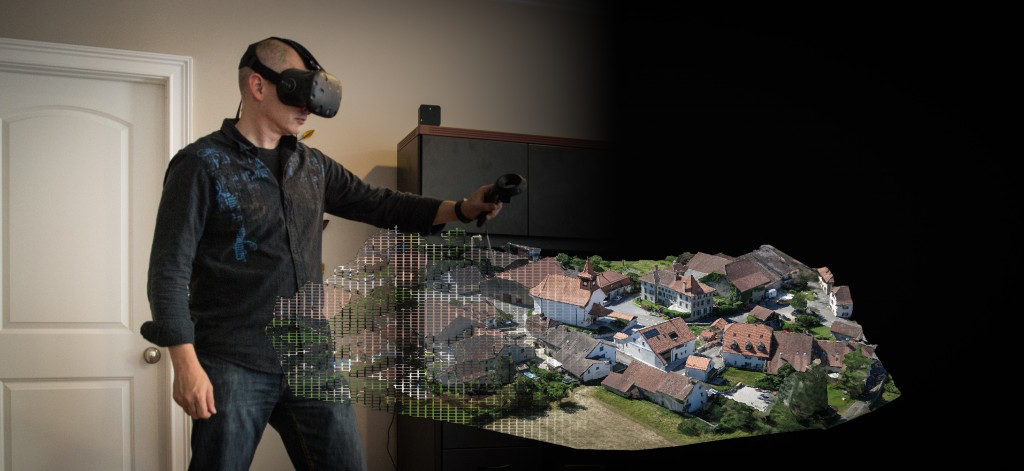
\includegraphics[width=3.5in]{images/ViveTownData.png}
%  \caption{HTC Vive Town using VTK with OpenVR.}
%  \label{fig:ViveTown}
%\end{figure}

\subsection{OpenVR Implementation}

This example creates a trivial VTK pipeline that reads a polygonal geometry file
using the \texttt{vtkPLYReader} and maps it to the scene using the above described \texttt{vtkOpenVR}
classes. As seen in Figure \ref{fig:openvrdragon}, the rendering
classes created a stereo pair from the view and warped it to the HTC Vive camera model. 
The example is available as a test case under the
\texttt{vtkOpenVR} module in the VTK source.

The modest amount of code needed to put VTK generated polygons into the
Vive HMD attests to the modularity and complete integration of the
existing VR framework|in this case, \texttt{vtkOpenVR}.

\begin{figure}[h!]
  \centering
  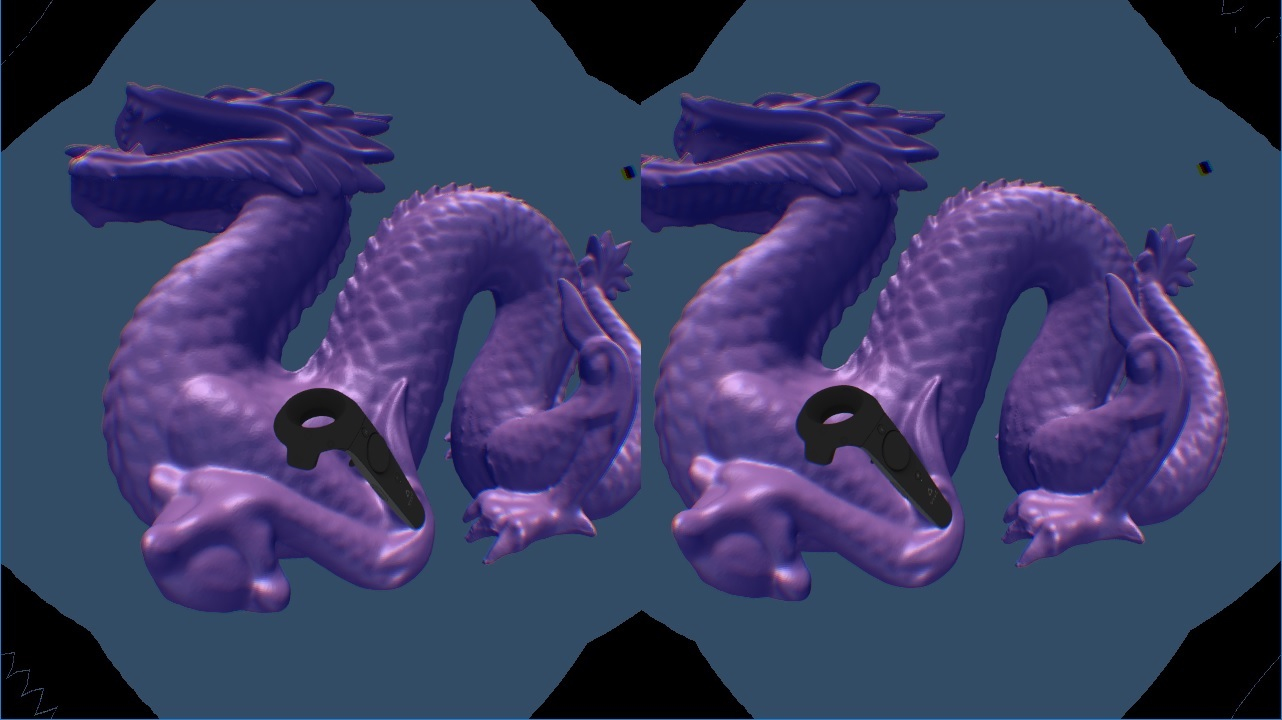
\includegraphics[width=3.in]{images/Dragon.jpg}
  \caption{A polygonal rendering of a sample dataset by VTK for OpenVR on HTC Vive.}
  \label{fig:openvrdragon}
\end{figure}

\section{Conclusion}

As the user base for virtual reality flourishes, there will be many
new users looking to use VR as a tool for scienctific visualization.
Rather than write new algorithms and tools entirely from scratch,
our extensions to the VTK system lowers the hurdles to cleanly
meld community-tested high-quality visualization algorithms into
existing VR integration libraries that can immersively render to
all-types of immersive systems, from large walk-in CAVE-style displays
to consumer-grade HMDs designed for games and game ecosystems (such
as SteamVR).

VTK has also been enhanced in ways that provide more efficient, and
therefore faster rendering | orders of magnitude faster in many cases.
Combined, we have moved VTK forward to where it can be \textbf{the}
tool of choice for immersive visualization development.


\section*{Acknowledgments}

The presented work was made possible due to support in part by funding from U.S. Department of Energy (Office of Nuclear Energy) Fast Track SBIR award DE-SC0010119, Dan Funk program manager, and from Idaho National Laboratory's Center for Advanced Energy Studies. Funding for embedding OpenVR, the OpenGL 3.2+ pipeline and SMP tools comes from the National Institutes of Health under the grant NIH R01EB014955 ``Accelerating Community-Driven Medical Innovation with VTK."


\bibliographystyle{abbrv}
\bibliography{VTK4IE}
\end{document}
